\chapter{Tạo các Docker Image}
\label{Chapter2}
Phần này sẽ hướng dẫn tạo và release các Docker Image tương ứng cho từng service sau.
\begin{enumerate}
    \item Service \texttt{{authenticaion}}
    \item Service \texttt{type-service}
    \item Service \texttt{record-service}
    \item Service \texttt{notification-service}
    \item Service \texttt{service-registry}
    \item Service \texttt{api-gateway}
    \item Ngoài ra, server \texttt{keycloak} cũng sẽ được tạo image riêng với cùng loại hướng dẫn.
\end{enumerate}

\section{Tạo file image}
Từ thư mục gốc \texttt{salesync} của mã nguồn. Truy cập vào thư mục \texttt{back-end} và truy cập thư mục con tương ứng với tên của service cần biên dịch.
Tiến hành chạy lệnh \\
\texttt{docker buildx build . -t tên-image:latest}\\
để Docker tìm đến file \texttt{Dockerfile} trong từng service và tiến hành tạo ra Container Image dựa trên file JAR trong thư mục \texttt{artifacts} đã chuẩn bị. Ta dùng argument \texttt{-t tên-image:latest} để đặt tên cho image trên máy tính, giúp thuận tiện hơn trong việc truy vấn.

Nếu thành công, kết quả trả về sẽ có dạng như Hình ~\ref{fig:docker_build_successfully}.

\begin{figure}
    \centering
    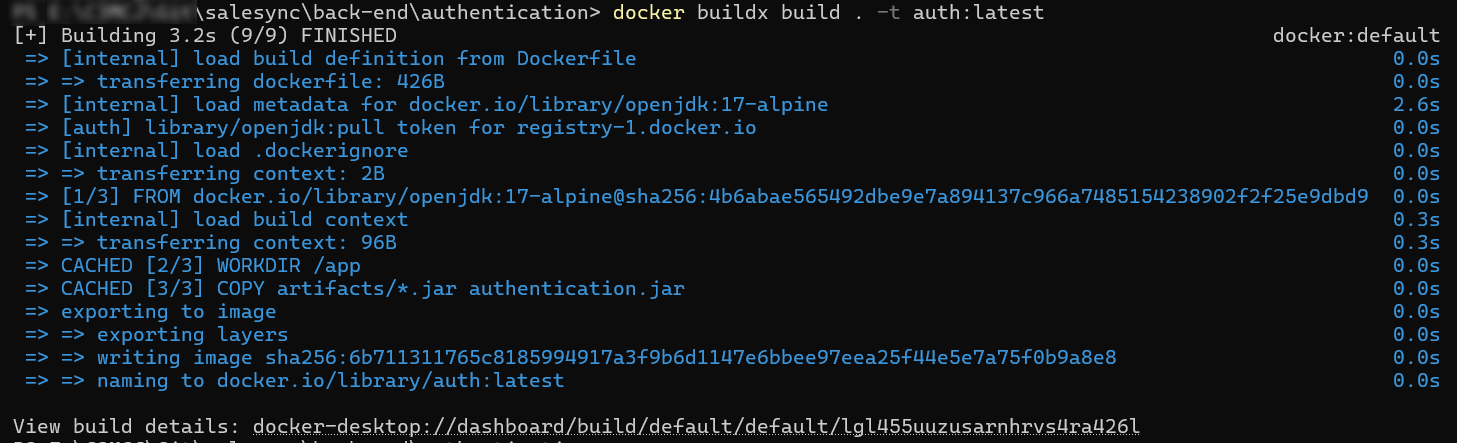
\includegraphics[width=1\linewidth]{docker_build_successfully.png}
    \caption{Docker đã tạo Image thành công}
    \label{fig:docker_build_successfully}
\end{figure}

\section{Đăng nhập vào Docker Hub (hoặc AWS ECR)}
\subsection{Docker Hub}
Đối với Docker Hub, chạy câu lệnh \texttt{docker login} và tiến hành nhập Username và password của tài khoản Docker Hub.

\subsection{AWS ECR}
Đối với AWS ECR, hướng dẫn này mặc định aws-cli đã được cài đặt và cấu hình trên máy tính (Xem hướng dẫn chi tiết tại \href{https://docs.aws.amazon.com/cli/latest/userguide/getting-started-install.html}{đây}). \\
Tương tự, ta cũng chạy lệnh đăng nhập đến AWS ECR, nhưng với cách thức lấy mật khẩu khác:

\texttt{docker login -u AWS -p \$(aws ecr get-login-password --region tên-region-aws) \\ mã-container-registry.dkr.ecr.ap-southeast-2.amazonaws.com}

\section{Tạo repository trên Docker Hub hoặc AWS ECR}
Dựa theo hướng dẫn riêng của từng container repository, ta cần tạo một repository trống để chứa image cho một service. Kết quả của quá trình này chính là một mã repository.

\section{Push Image lên Docker Hub hoặc AWS ECR}
Trước tiên, ta cần gán tag để image vừa build tại máy tính đến tên repository đã tạo.

\texttt{docker tag tên-image:latest mã-repository:latest}

Sau đó, chạy lệnh sau để push image lên repository.
\texttt{docker push mã-repository:latest}

\textbf{\textit{Chú ý}}: Trong những bước đã liệt kê, có thể thay đỏi tag \texttt{latest} thành tên của số hiệu phiên bản mong muốn.


\section{Lặp lại với các service khác}
Thực hiện những bước tương tự với các service khác, kết quả đạt được bao gồm $6$ repository khác nhau tương ứng với $6$ service đã liệt kê. Đây cũng là sản phẩm cuối cùng của quy trình tạo và release image.